% Options for packages loaded elsewhere
\PassOptionsToPackage{unicode}{hyperref}
\PassOptionsToPackage{hyphens}{url}
%
\documentclass[
  9pt,
  ignorenonframetext,
]{beamer}
\usepackage{pgfpages}
\setbeamertemplate{caption}[numbered]
\setbeamertemplate{caption label separator}{: }
\setbeamercolor{caption name}{fg=normal text.fg}
\beamertemplatenavigationsymbolsempty
% Prevent slide breaks in the middle of a paragraph
\widowpenalties 1 10000
\raggedbottom
\setbeamertemplate{part page}{
  \centering
  \begin{beamercolorbox}[sep=16pt,center]{part title}
    \usebeamerfont{part title}\insertpart\par
  \end{beamercolorbox}
}
\setbeamertemplate{section page}{
  \centering
  \begin{beamercolorbox}[sep=12pt,center]{part title}
    \usebeamerfont{section title}\insertsection\par
  \end{beamercolorbox}
}
\setbeamertemplate{subsection page}{
  \centering
  \begin{beamercolorbox}[sep=8pt,center]{part title}
    \usebeamerfont{subsection title}\insertsubsection\par
  \end{beamercolorbox}
}
\AtBeginPart{
  \frame{\partpage}
}
\AtBeginSection{
  \ifbibliography
  \else
    \frame{\sectionpage}
  \fi
}
\AtBeginSubsection{
  \frame{\subsectionpage}
}
\usepackage{lmodern}
\usepackage{amsmath}
\usepackage{ifxetex,ifluatex}
\ifnum 0\ifxetex 1\fi\ifluatex 1\fi=0 % if pdftex
  \usepackage[T1]{fontenc}
  \usepackage[utf8]{inputenc}
  \usepackage{textcomp} % provide euro and other symbols
  \usepackage{amssymb}
\else % if luatex or xetex
  \usepackage{unicode-math}
  \defaultfontfeatures{Scale=MatchLowercase}
  \defaultfontfeatures[\rmfamily]{Ligatures=TeX,Scale=1}
\fi
\usetheme[]{Goettingen}
\usecolortheme{rose}
% Use upquote if available, for straight quotes in verbatim environments
\IfFileExists{upquote.sty}{\usepackage{upquote}}{}
\IfFileExists{microtype.sty}{% use microtype if available
  \usepackage[]{microtype}
  \UseMicrotypeSet[protrusion]{basicmath} % disable protrusion for tt fonts
}{}
\makeatletter
\@ifundefined{KOMAClassName}{% if non-KOMA class
  \IfFileExists{parskip.sty}{%
    \usepackage{parskip}
  }{% else
    \setlength{\parindent}{0pt}
    \setlength{\parskip}{6pt plus 2pt minus 1pt}}
}{% if KOMA class
  \KOMAoptions{parskip=half}}
\makeatother
\usepackage{xcolor}
\IfFileExists{xurl.sty}{\usepackage{xurl}}{} % add URL line breaks if available
\IfFileExists{bookmark.sty}{\usepackage{bookmark}}{\usepackage{hyperref}}
\hypersetup{
  pdftitle={BIOS6643 Longitudinal},
  pdfauthor={EJC},
  hidelinks,
  pdfcreator={LaTeX via pandoc}}
\urlstyle{same} % disable monospaced font for URLs
\newif\ifbibliography
\setlength{\emergencystretch}{3em} % prevent overfull lines
\providecommand{\tightlist}{%
  \setlength{\itemsep}{0pt}\setlength{\parskip}{0pt}}
\setcounter{secnumdepth}{-\maxdimen} % remove section numbering
\AtBeginSubsection{}
\AtBeginSection{}
\ifluatex
  \usepackage{selnolig}  % disable illegal ligatures
\fi

\title{BIOS6643 Longitudinal}
\subtitle{L8 Covariance}
\author{EJC}
\date{}
\institute{Department of Biostatistics ~~ Informatics}

\begin{document}
\frame{\titlepage}

\begin{frame}[allowframebreaks]
  \tableofcontents[hideallsubsections]
\end{frame}
\hypertarget{covariance-structure}{%
\section{Covariance Structure}\label{covariance-structure}}

\begin{frame}{Topics for today (Advanced covariance structures):}
\protect\hypertarget{topics-for-today-advanced-covariance-structures}{}
\begin{itemize}
\item
  Recap from last lecture: Mt. K data and fit with random effects; some
  unusual results: non-positive definite G; partial random effect
  results; model still usable?
\item
  Quick review of \(\pmb R\) structures, up to Kronecker Product
\item
  Modeling \(\pmb G\) and \(\pmb R\) simultaneously
\item
  Another look at Mt. K data, several modeling approaches.
\item
  Fitting a joint normal outcome using a mixed model!
\end{itemize}

\vspace{\baselineskip}

\textbf{Reading: Relevant sections from the LMM course notes.}
\end{frame}

\begin{frame}{Recap of \(R_i\) structures for, say, 4 measures}
\protect\hypertarget{recap-of-r_i-structures-for-say-4-measures}{}
\begin{itemize}
\tightlist
\item
  Simple
\end{itemize}

\vspace{\baselineskip}
\vspace{\baselineskip}

\begin{itemize}
\tightlist
\item
  CS
\end{itemize}

\vspace{\baselineskip}
\vspace{\baselineskip}

\begin{itemize}
\tightlist
\item
  UN
\end{itemize}

\vspace{\baselineskip}
\vspace{\baselineskip}

\begin{itemize}
\tightlist
\item
  AR(1)
\end{itemize}

\vspace{\baselineskip}
\vspace{\baselineskip}

\begin{itemize}
\tightlist
\item
  Spatial power
\end{itemize}

\vspace{\baselineskip}
\vspace{\baselineskip}

Many others, but the above are ones I most commonly use. For `CS', I
usually just a random intercept, in which case you don't need to
additionally specify CS for the \(\pmb R\) structure.
\end{frame}

\hypertarget{kronecker-product}{%
\section{Kronecker Product}\label{kronecker-product}}

\begin{frame}{Kronecker Product}
\protect\hypertarget{kronecker-product-1}{}
Modeling doubly repeated measures via the error covariance (R) matrix
using the Direct Product (Kronecker) structure

\begin{itemize}
\item
  For some data sets, we may need to account for repeated measures over
  two dimensions.
\item
  For example, say that strength measurements are taken on each leg for
  subjects over 3 time points. There are 2 `repeated measures' in space
  (i.e., body part) as well as 3 repeated measures over time.
\item
  The covariance matrix to account for all repeated measures would then
  have size \(6 \times 6\).
\item
  Instead of dealing with this big messy matrix, it is easier to define
  it in pieces and then take the Kronecker product.
\end{itemize}
\end{frame}

\begin{frame}{}
\protect\hypertarget{section}{}
\begin{block}{\textbf{Example 1}:}
\protect\hypertarget{example-1}{}
For the scenario described above, say that repeated measures over space
can be modeled with the UN structure and repeated measures over time can
be modeled with the AR(1) structure:

Structure for space: \[
R_{i1} = 
\begin{pmatrix}
\sigma_1^2\ \sigma_{12}\\
\sigma_{12}\ \sigma_2^2     
\end{pmatrix}
\]

Structure for time:

\[
R_{i2} = \sigma_\epsilon^2
\begin{pmatrix} 
1 \ \ \phi \ \ \phi^2 \\
\phi \ \ 1 \ \ \phi \\
\phi^2 \ \ \phi \ \ 1
\end{pmatrix}
\]
\end{block}
\end{frame}

\begin{frame}{}
\protect\hypertarget{section-1}{}
The combined (Kronecker product structure):

\begin{block}{\textbf{Example 1}}
\protect\hypertarget{example-1-1}{}
\[
R_i = R_{i1}\otimes R_{i2} =
\begin{pmatrix}
\sigma_1^2 \ \ \sigma_{12}\\ 
\sigma_{12}\ \ \sigma_2^2 
\end{pmatrix}
\otimes \sigma_\epsilon^2 
\begin{pmatrix}
1 \ \ \phi \ \ \phi^2 \\
\phi \ \ 1 \ \ \phi \\
\phi^2 \ \ \phi \ \ 1
\end{pmatrix}
=\begin{pmatrix}
\sigma_1^2 R_{i2} \ \ \sigma_{12}  R_{i2} \\ 
\sigma_{12}  R_{i2} \ \ \sigma_2^2 R_{i2} 
\end{pmatrix}
\]

\[ 
= \begin{pmatrix}
\sigma_1^2
\begin{pmatrix}
 1 \ \ \phi \ \ \phi^2 \\ 
 \phi \ \ 1 \ \ \phi \\ 
 \phi^2 \ \ \phi \ \ 1
\end{pmatrix}
\ \ \ \
\sigma_{12} 
\begin{pmatrix}
 1 \ \ \phi \ \ \phi^2 \\ 
 \phi \ \ 1 \ \ \phi \\ 
 \phi^2 \ \ \phi \ \ 1
\end{pmatrix}\\
\sigma_{12}
\begin{pmatrix}
 1 \ \ \phi \ \ \phi^2 \\ 
 \phi \ \ 1 \ \ \phi \\ 
 \phi^2 \ \ \phi \ \ 1
\end{pmatrix}
\ \ \ \
\sigma_2^2 
\begin{pmatrix}
 1 \ \ \phi \ \ \phi^2 \\ 
 \phi \ \ 1 \ \ \phi \\ 
 \phi^2 \ \ \phi \ \ 1
\end{pmatrix}
\end{pmatrix}
\]

\[
= \begin{pmatrix}
\sigma_1^2 \ \ \ \ \sigma_1^2 \phi \ \ \ \ \sigma_1^2 \phi^2  \ \ \ \ \sigma_{12}\ \ \ \ \sigma_{12}\phi \ \ \ \ \sigma_{12}\phi^2 \\ 
\sigma_1^2 \phi \ \ \ \ \sigma_1^2 \ \ \ \ \sigma_1^2 \phi \ \ \ \ \sigma_{12}\phi \ \ \ \ \sigma_{12}\ \ \ \ \sigma_{12}\phi \\ 
\sigma_1^2 \phi^2 \ \ \ \ \sigma_1^2 \phi \ \ \ \ \sigma_1^2 \ \ \ \ \sigma_{12}\phi^2 \ \ \ \ \ \sigma_{12}\phi \ \ \ \ \sigma_{12}\\ 
\sigma_{12}\ \ \ \ \sigma_{12}\phi \ \ \ \ \sigma_{12}\phi^2 \ \ \ \ \sigma_2^2 \ \ \ \ \sigma_2^2 \phi \ \ \ \ \sigma_2^2 \phi^2 \\ 
\sigma_{12}\phi \ \ \ \ \sigma_{12}\ \ \ \ \sigma_{12}\phi \ \ \ \ \sigma_2^2 \phi \ \ \ \ \sigma_2^2 \ \ \ \ \sigma_2^2 \phi \\ 
\sigma_{12}\phi^2 \ \ \ \ \sigma_{12}\phi \ \ \ \ \sigma_{12}\ \ \ \ \sigma_2^2 \phi^2 \ \ \ \ \sigma_2^2 \phi \ \ \ \ \sigma_2^2
\end{pmatrix} 
\]
\end{block}
\end{frame}

\begin{frame}{}
\protect\hypertarget{section-2}{}
Note: the \(\sigma_\epsilon^2\) on the AR(1) structure is not included
because it becomes redundant once we take the direct product, i.e., it
is absorbed into parameters in the other matrix. Available Kronecker
structures in SAS include: \(UN @ AR(1)\), \(UN @ CS\) and \(UN @ UN\).
(The symbol `\(@\)' is used to denote `\(\otimes\)' since the latter is
not on the keyboard!)

\begin{block}{\textbf{Example 2}}
\protect\hypertarget{example-2}{}
Measuring cortisol 3 times a day, for 7 successive days.

\vspace{\baselineskip}
\vspace{\baselineskip}
\vspace{\baselineskip}
\vspace{\baselineskip}
\vspace{\baselineskip}
\vspace{\baselineskip}
\vspace{\baselineskip}
\vspace{\baselineskip}
\vspace{\baselineskip}
\vspace{\baselineskip}
\end{block}
\end{frame}

\begin{frame}{Some things to remember about covariance matrices in mixed
models:}
\protect\hypertarget{some-things-to-remember-about-covariance-matrices-in-mixed-models}{}
\begin{itemize}
\item
  \(Cov[\pmb Y]\) or
  \(Var[\pmb Y] = \pmb V = \pmb {ZGZ}^{\top} + \pmb R\)
\item
  If no random effects, then \(Cov[\pmb Y] = Cov[\pmb \epsilon]\), i.e.,
  \(\pmb V= \pmb R\).
\item
  Since the \(Cov[\pmb Y]\) is of primary interest, this formula
  suggests there are different ways to account for correlated data,
  through \(\pmb R\) (the covariance matrix of the errors), through
  \(\pmb G\) (The covariance matrix of random effects) or both.
\end{itemize}
\end{frame}

\begin{frame}{Putting it together:}
\protect\hypertarget{putting-it-together}{}
Specifying \(\pmb G\) and \(\pmb R\) in the same model

\begin{itemize}
\item
  So far we've discussed how you can either specify \(\pmb G\) or
  \(\pmb R\) in fitting a mixed model. However, you can actually do
  both, which may be advantageous for some data.
\item
  Recall the Mt. Kilimanjaro data. By including up to quadratic random
  effects, we can actually develop an altitude-sensitive covariance
  structure that allows the correlation to decrease as altitude between
  measurements increases. (Altitude and time are closely related.)
\item
  We can also directly model the repeated measures through \(\pmb R\).
  (Although repeated measures are not likely to be exactly equally
  spaced, we do not have exact times of measurement, so the AR(1) will
  have to do.) or, we can do both!
\end{itemize}
\end{frame}

\hypertarget{mt.-k-data}{%
\section{Mt. K data}\label{mt.-k-data}}

\begin{frame}{}
\protect\hypertarget{section-3}{}
Quick aside: what do Mt. K data look like? (\(x = altitude, km\))

\begin{center}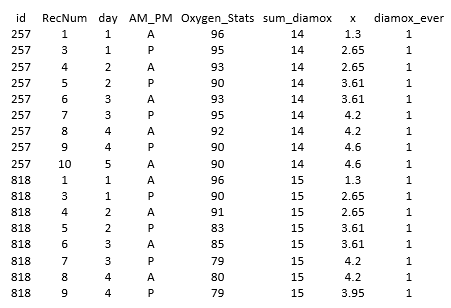
\includegraphics[width=1\linewidth]{figs_L8/f1} \end{center}
\end{frame}

\begin{frame}{Modeling approaches for Mt. K data:}
\protect\hypertarget{modeling-approaches-for-mt.-k-data}{}
\begin{itemize}
\item
  Approach 1: random + simple \(\pmb R\) (i.e., \(R=\sigma^2 \pmb I\)).

  \begin{itemize}
  \tightlist
  \item
    We did this already (see last slide set).
  \item
    AIC=69599.3

    \begin{itemize}
    \tightlist
    \item
      Correlation parameter estimate is \(\sim\) 0.08 (estimated
      correlation between two errors 0.5 day apart, not responses).
    \end{itemize}
  \end{itemize}
\item
  Approach 2: random + AR(1) structure for R.
\item
  AIC=69545.2 (54 point drop). Both \(\pmb G\) and \(\pmb R\) contribute
  to the covariance structure:
  \(\pmb V=Var[\pmb Y]=\pmb {ZGZ}^{\top} + \pmb R\).
\end{itemize}

\begin{center}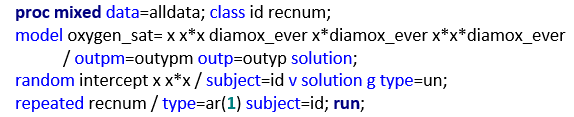
\includegraphics[width=0.7\linewidth]{figs_L8/f2} \end{center}
\end{frame}

\begin{frame}{Some other possibilities:}
\protect\hypertarget{some-other-possibilities}{}
\begin{itemize}
\item
  Approach 3: Remove RANDOM statement so that \(\pmb V= \pmb R\).

  \begin{itemize}
  \item
    The estimated correlation parameter (which now does represent the
    correlation between responses 0.5 day apart) in the structure
    increases to \(\sim\) 0.44.
  \item
    This is because the random effects no longer contribute to the
    covariance between 2 responses, I.e., to get roughly the same
    covariance between 2 responses, the contribution from \(\pmb R\)
    needs to increase since there is no longer a contribution from
    \(\pmb {ZGZ}^{\top}\).
  \item
    AIC increases A LOT.
  \end{itemize}
\item
  Approach 4: Up to linear random effects, simple R.

  \begin{itemize}
  \tightlist
  \item
    AIC also high
  \end{itemize}
\item
  Approach 5: Quadratic random effects plus Kronecker Product structure
  for errors.

  \begin{itemize}
  \item
    Really complicated model! But AIC good.
  \item
    Model makes intuitive sense.
  \end{itemize}
\end{itemize}
\end{frame}

\begin{frame}{AIC values for different covariance structure approaches.}
\protect\hypertarget{aic-values-for-different-covariance-structure-approaches.}{}
\begin{center}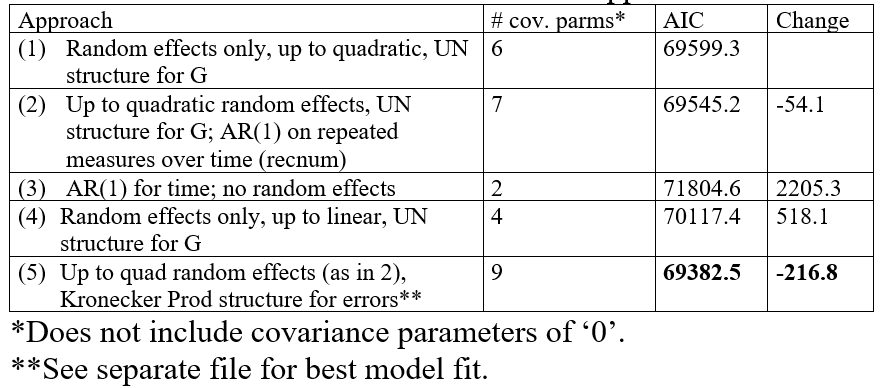
\includegraphics[width=0.7\linewidth]{figs_L8/f3} \end{center}

In comparing AIC, make sure same number of records used! For these fits,
\(n=13,368\) used (1 missing value due to loss of info in am\_pm and day
variables)
\end{frame}

\begin{frame}{}
\protect\hypertarget{section-4}{}
For applications in which the random effects are defined on time rather
some other variable (such as altitude, above), including a non-simple
structure for time via \(\pmb R\) may still improve the model fit.

\begin{itemize}
\item
  For example, an outcome for which there is substantial between-subject
  heterogeneity (not accounted for in the predictors), but with repeated
  measures over time might require a random intercept plus an AR(1)
  structure for \(\pmb R\).
\item
  Generally, it is recommended to first narrow the list of possible
  covariance structures, followed by a comparison of goodness-of-fit
  values for these possibilities.
\end{itemize}
\end{frame}

\hypertarget{fitting-joint-normal-outcomes-using-mixed-models}{%
\section{Fitting joint normal outcomes using mixed
models}\label{fitting-joint-normal-outcomes-using-mixed-models}}

\begin{frame}{Fitting joint normal outcomes using mixed models}
\protect\hypertarget{fitting-joint-normal-outcomes-using-mixed-models-1}{}
\begin{itemize}
\item
  Let's say we have 2 outcomes with different units, and measurements
  over time for each of these. Can we use mixed models in this case?
  Sure, but proceed with caution!
\item
  For simplicity, consider the COPDGene data, which has 2 measurements
  taken on subjects with COPD (GOLD groups 2 through 4) that are about 5
  years apart. The 2 outcomes to be considered are FEV1 (a pulmonary
  function measure) and distance walked (an exercise ability measure).
\item
  The original data set has FEV1 and distance walked in separate
  columns. In order to fit the model, we need to create a new, composite
  variable, call it y, and then create a variable, call it type, to
  identify when y is FEV1 and when y is distance walked (dist for short)
\end{itemize}

\begin{center}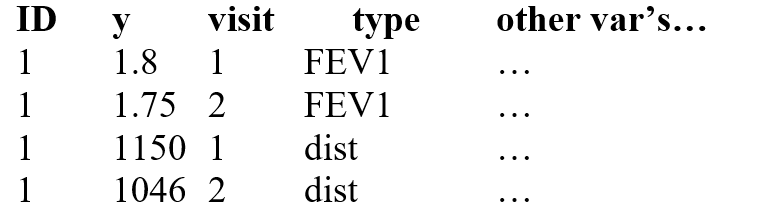
\includegraphics[width=0.5\linewidth]{figs_L8/f4} \end{center}
\end{frame}

\begin{frame}{}
\protect\hypertarget{section-5}{}
\begin{itemize}
\tightlist
\item
  FEV1 is measured in liters, and is usally around 1 to 3, while
  distance walked is in feet, for a 6-minte time frame and is usually
  over 1000.
\end{itemize}

The SAS code to fit the model:

\begin{center}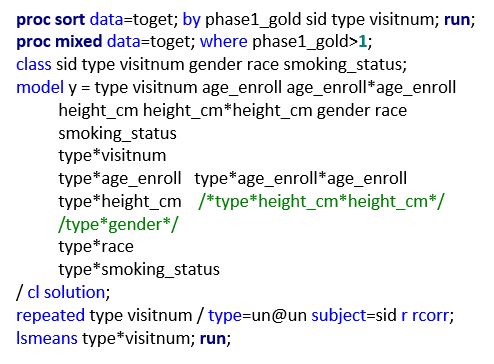
\includegraphics[width=1\linewidth]{figs_L8/f5} \end{center}
\end{frame}

\begin{frame}{}
\protect\hypertarget{section-6}{}
\begin{itemize}
\item
  Ideally the list of covariates (i.e., terms other than type or
  visitnum) should include variables that are important to either FEV1
  or distance walked. Also, I started with a model that included all
  possible interactions between type and other covariates; I later
  dropped \(type \times height^2\) and \(type \times gender\) due to
  very weak significance. The \(visitnum \times type\) term is important
  to keep in the model, regardless of significance.
\item
  It is important to remember that if we drop a particular
  \(type \times covariate\) interaction, then we're assuming the
  relationship between that covariate and FEV1 can share the same slope
  as for the covariate and distance walked. When the units between the
  outcome types differ, this may be a tall order, and is why I start
  with a model that includes all possible interactions.
\end{itemize}
\end{frame}

\begin{frame}{Selected output:}
\protect\hypertarget{selected-output}{}
\begin{center}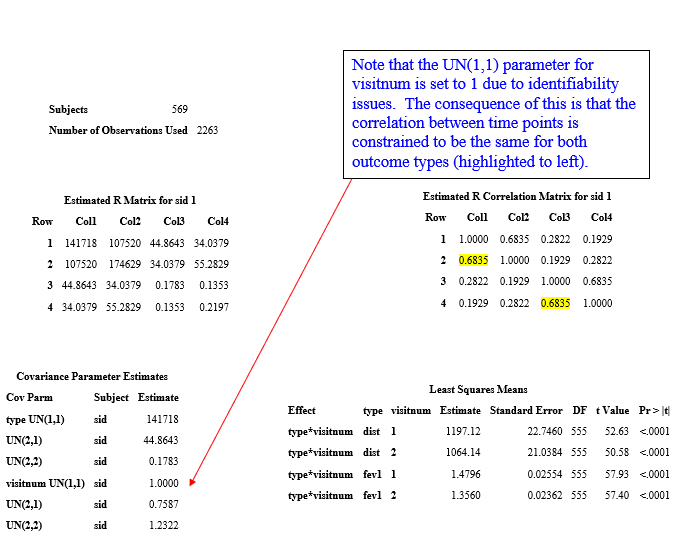
\includegraphics[width=1\linewidth]{figs_L8/f6} \end{center}
\end{frame}

\begin{frame}{}
\protect\hypertarget{section-7}{}
\begin{itemize}
\item
  If we fit FEV1 and distance walked in separate model, the correlation
  between time points for FEV1 is 0.82 and for dist is 0.55; this
  explains the `pooled' correlation of 0.68 when modeling the outcomes
  jointly.
\item
  Least-squares means estimates and SE's are similar when running
  individually as when running jointly. The joint model has slightly
  higher SE's for distance walked and slightly lower SE's for FEV1 due
  to model constraints.
\end{itemize}

\begin{center}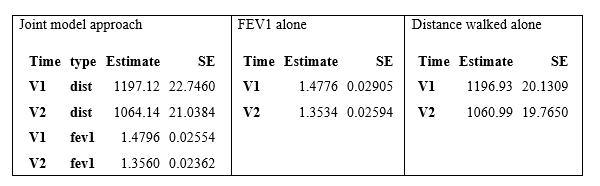
\includegraphics[width=1\linewidth]{figs_L8/f7} \end{center}
\end{frame}

\hypertarget{some-notes}{%
\section{Some notes}\label{some-notes}}

\begin{frame}{Notes}
\protect\hypertarget{notes}{}
\begin{itemize}
\item
  The major advantage of running models with FEV1 and distance walked
  together is to better understand correlation between them, while
  simultaneously conducting inference for effects of interest, which is
  how the outcomes change over time.
\item
  If the two outcomes being measured actually have the same units, then
  it may simplify the model, with respect to both the necessary
  predictors (including interaction terms) and the suitable covariance
  structure.
\item
  For outcomes that are measured in different units, an alternative to
  modeling them in raw units is to standardize the outcomes in some
  fashion, which might simplify the necessary predictors and interaction
  terms. For example, FEV1 is sometimes put into `percent of predicted'
  terms based on age, height gender and race (in some cases using
  squared terms for continuous variables). If a similar approach is used
  for distance walked, then the list of predictors reduces to type and
  visit (and their interaction).
\item
  We could try the UN structure for the complete list of repeated
  measures. This would introduce 10 covariance parameters; a very
  flexible matrix but harder to fit and possibly introduces more
  parameters than necessary. In the case of the data above, it did not
  converge.
\end{itemize}
\end{frame}

\hypertarget{summary}{%
\section{Summary}\label{summary}}

\begin{frame}{Summary}
\protect\hypertarget{summary-1}{}
\end{frame}

\end{document}
